\subsection{Approach}

\label{sys:appr}
We took a black-box approach to measure the prevalence of \ehi
vulnerabilities on the web. Black-box
testing~\cite{Beizer:1995:BTT:202699} is a way to examine the
functionality of an application without analyzing its source code. Black-box testing allows our system to detect \ehi vulnerabilities in \emph{any} server-side language (not simply those we identified in Section~\ref{languages}). The overall architecture of our system is presented in Figure~\ref{fig:overall}. 

%\begin{wrapfigure}{r}{6.5cm}
\begin{figure}[tb]
	\centering
	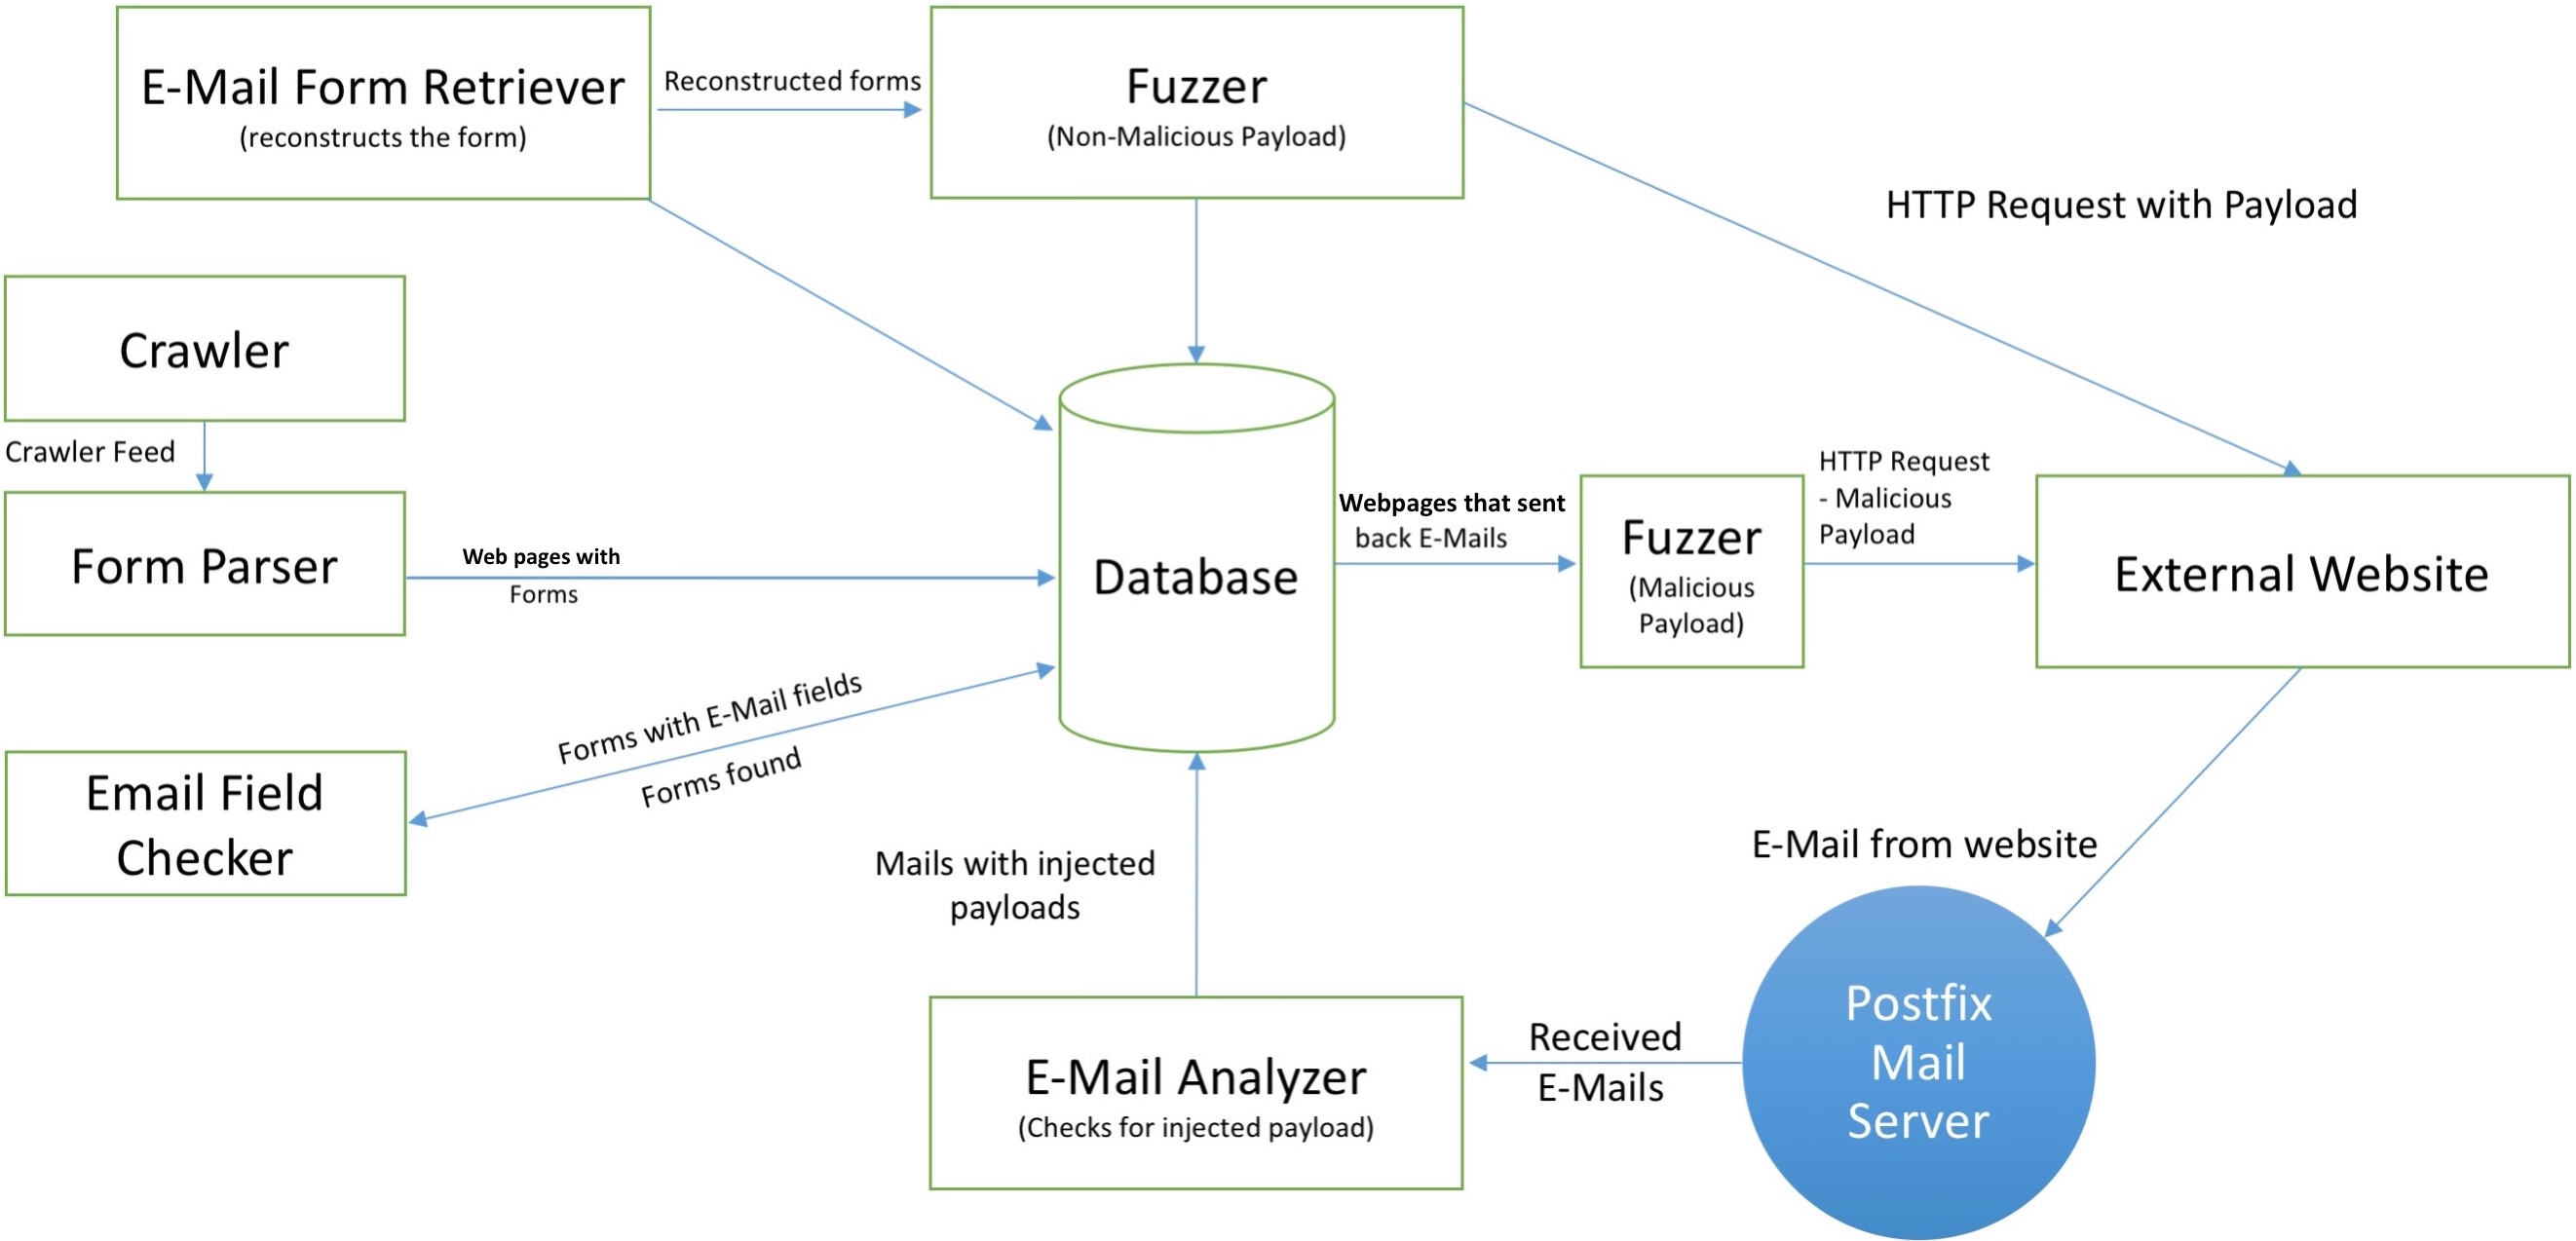
\includegraphics[width=.5\textwidth]{overall_crop}
	\caption{Overall system architecture.}
    
	\label{fig:overall}
\end{figure}
%\end{wrapfigure}
